\documentclass[mathserif]{beamer}
\usepackage{amsmath}
\usepackage{color}
\usepackage{amsfonts}
\usepackage{xcolor,graphicx}
\usepackage{geometry}
\usepackage{hyperref}
\usepackage{mathrsfs}

\title{Forecasting Stocks}
\author{Brady Metherall}
\date{Wednesday November 29, 2017}

\usetheme{Berkeley}
\usecolortheme{whale}

\begin{document}
\frame{\titlepage}
\setlength\parindent{0pt}

\section{Black-Scholes Model}

\frame{
\frametitle{Black-Scholes Model}
To generate data the Black-Scholes model was used. The Black-Scholes model is a mathematical model for the financial market. It is defined by the stochastic differential equation
\begin{align*}
dS &= \mu S dt + \sigma S dW_t,
\end{align*}
where $\mu$ is the trend, $\sigma$ the variance / volatility, and $W_t$ is a Brownian motion. This can be discretized as
\begin{align*}
S_{t+1} &= S_t \left( 1 + \mu \Delta t + \sigma \mathcal{N}(0,1) \sqrt{\Delta t} \right).
\end{align*}
}

\frame{
\frametitle{Black-Scholes Model}
However, historical financial data is only available on a day-to-day basis. To have similar data, we let $\Delta t = 1$ min. so that $1440 \Delta t = 1$ day. And so, the open, close, min, and max can be extracted in each block of 1440 time steps.
}

\frame{
\frametitle{Black-Scholes Model}
\begin{figure}
% GNUPLOT: LaTeX picture with Postscript
\begingroup
  \makeatletter
  \providecommand\color[2][]{%
    \GenericError{(gnuplot) \space\space\space\@spaces}{%
      Package color not loaded in conjunction with
      terminal option `colourtext'%
    }{See the gnuplot documentation for explanation.%
    }{Either use 'blacktext' in gnuplot or load the package
      color.sty in LaTeX.}%
    \renewcommand\color[2][]{}%
  }%
  \providecommand\includegraphics[2][]{%
    \GenericError{(gnuplot) \space\space\space\@spaces}{%
      Package graphicx or graphics not loaded%
    }{See the gnuplot documentation for explanation.%
    }{The gnuplot epslatex terminal needs graphicx.sty or graphics.sty.}%
    \renewcommand\includegraphics[2][]{}%
  }%
  \providecommand\rotatebox[2]{#2}%
  \@ifundefined{ifGPcolor}{%
    \newif\ifGPcolor
    \GPcolortrue
  }{}%
  \@ifundefined{ifGPblacktext}{%
    \newif\ifGPblacktext
    \GPblacktexttrue
  }{}%
  % define a \g@addto@macro without @ in the name:
  \let\gplgaddtomacro\g@addto@macro
  % define empty templates for all commands taking text:
  \gdef\gplbacktext{}%
  \gdef\gplfronttext{}%
  \makeatother
  \ifGPblacktext
    % no textcolor at all
    \def\colorrgb#1{}%
    \def\colorgray#1{}%
  \else
    % gray or color?
    \ifGPcolor
      \def\colorrgb#1{\color[rgb]{#1}}%
      \def\colorgray#1{\color[gray]{#1}}%
      \expandafter\def\csname LTw\endcsname{\color{white}}%
      \expandafter\def\csname LTb\endcsname{\color{black}}%
      \expandafter\def\csname LTa\endcsname{\color{black}}%
      \expandafter\def\csname LT0\endcsname{\color[rgb]{1,0,0}}%
      \expandafter\def\csname LT1\endcsname{\color[rgb]{0,1,0}}%
      \expandafter\def\csname LT2\endcsname{\color[rgb]{0,0,1}}%
      \expandafter\def\csname LT3\endcsname{\color[rgb]{1,0,1}}%
      \expandafter\def\csname LT4\endcsname{\color[rgb]{0,1,1}}%
      \expandafter\def\csname LT5\endcsname{\color[rgb]{1,1,0}}%
      \expandafter\def\csname LT6\endcsname{\color[rgb]{0,0,0}}%
      \expandafter\def\csname LT7\endcsname{\color[rgb]{1,0.3,0}}%
      \expandafter\def\csname LT8\endcsname{\color[rgb]{0.5,0.5,0.5}}%
    \else
      % gray
      \def\colorrgb#1{\color{black}}%
      \def\colorgray#1{\color[gray]{#1}}%
      \expandafter\def\csname LTw\endcsname{\color{white}}%
      \expandafter\def\csname LTb\endcsname{\color{black}}%
      \expandafter\def\csname LTa\endcsname{\color{black}}%
      \expandafter\def\csname LT0\endcsname{\color{black}}%
      \expandafter\def\csname LT1\endcsname{\color{black}}%
      \expandafter\def\csname LT2\endcsname{\color{black}}%
      \expandafter\def\csname LT3\endcsname{\color{black}}%
      \expandafter\def\csname LT4\endcsname{\color{black}}%
      \expandafter\def\csname LT5\endcsname{\color{black}}%
      \expandafter\def\csname LT6\endcsname{\color{black}}%
      \expandafter\def\csname LT7\endcsname{\color{black}}%
      \expandafter\def\csname LT8\endcsname{\color{black}}%
    \fi
  \fi
    \setlength{\unitlength}{0.0500bp}%
    \ifx\gptboxheight\undefined%
      \newlength{\gptboxheight}%
      \newlength{\gptboxwidth}%
      \newsavebox{\gptboxtext}%
    \fi%
    \setlength{\fboxrule}{0.5pt}%
    \setlength{\fboxsep}{1pt}%
\begin{picture}(5760.00,3844.00)%
    \gplgaddtomacro\gplbacktext{%
      \csname LTb\endcsname%
      \put(814,704){\makebox(0,0)[r]{\strut{}$0.8$}}%
      \csname LTb\endcsname%
      \put(814,1115){\makebox(0,0)[r]{\strut{}$1$}}%
      \csname LTb\endcsname%
      \put(814,1525){\makebox(0,0)[r]{\strut{}$1.2$}}%
      \csname LTb\endcsname%
      \put(814,1936){\makebox(0,0)[r]{\strut{}$1.4$}}%
      \csname LTb\endcsname%
      \put(814,2347){\makebox(0,0)[r]{\strut{}$1.6$}}%
      \csname LTb\endcsname%
      \put(814,2758){\makebox(0,0)[r]{\strut{}$1.8$}}%
      \csname LTb\endcsname%
      \put(814,3168){\makebox(0,0)[r]{\strut{}$2$}}%
      \csname LTb\endcsname%
      \put(814,3579){\makebox(0,0)[r]{\strut{}$2.2$}}%
      \csname LTb\endcsname%
      \put(946,484){\makebox(0,0){\strut{}$0$}}%
      \csname LTb\endcsname%
      \put(1388,484){\makebox(0,0){\strut{}$2$}}%
      \csname LTb\endcsname%
      \put(1829,484){\makebox(0,0){\strut{}$4$}}%
      \csname LTb\endcsname%
      \put(2271,484){\makebox(0,0){\strut{}$6$}}%
      \csname LTb\endcsname%
      \put(2713,484){\makebox(0,0){\strut{}$8$}}%
      \csname LTb\endcsname%
      \put(3155,484){\makebox(0,0){\strut{}$10$}}%
      \csname LTb\endcsname%
      \put(3596,484){\makebox(0,0){\strut{}$12$}}%
      \csname LTb\endcsname%
      \put(4038,484){\makebox(0,0){\strut{}$14$}}%
      \csname LTb\endcsname%
      \put(4480,484){\makebox(0,0){\strut{}$16$}}%
      \csname LTb\endcsname%
      \put(4921,484){\makebox(0,0){\strut{}$18$}}%
      \csname LTb\endcsname%
      \put(5363,484){\makebox(0,0){\strut{}$20$}}%
    }%
    \gplgaddtomacro\gplfronttext{%
      \csname LTb\endcsname%
      \put(176,2141){\rotatebox{-270}{\makebox(0,0){\strut{}Stock Price}}}%
      \put(3154,154){\makebox(0,0){\strut{}Time $\left( \text{Days} \times 10^3 \right)$}}%
    }%
    \gplbacktext
    \put(0,0){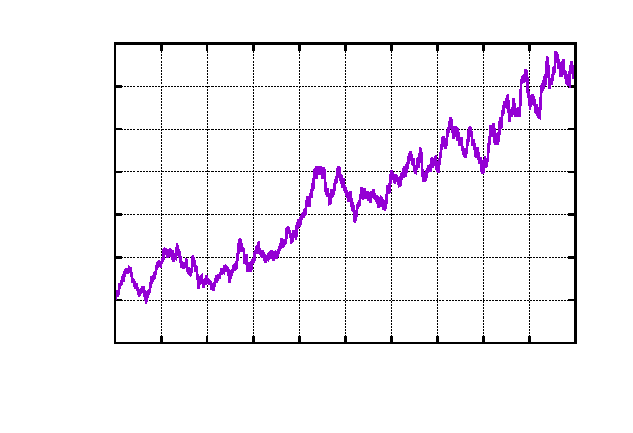
\includegraphics{ToyStock}}%
    \gplfronttext
  \end{picture}%
\endgroup

\end{figure}
}

\section{Network}

\frame{
\frametitle{Network}
Network Parameters:
\begin{tabular}{l l l}
Parameter & First Layer & Second Layer \\
\hline
Type & LSTM & Fully Connected \\
Number of Neurons & 64 & 5 \\
Activation & Tanh & Tanh \\
Dropout & 10\% & N/A
\end{tabular} \\
\vspace{4mm}
Training Parameters:
\begin{tabular}{l l}
Parameter & Value \\
\hline
Loss & Mean Absolute Percent Error \\
Optimizer & Adam \\
Window & 15 \\
Batch Size & 64 \\
Validation & 20\% \\
Epochs & 50
\end{tabular}
}

\frame{
\frametitle{Regular Normalization}
\begin{figure}
% GNUPLOT: LaTeX picture with Postscript
\begingroup
  \makeatletter
  \providecommand\color[2][]{%
    \GenericError{(gnuplot) \space\space\space\@spaces}{%
      Package color not loaded in conjunction with
      terminal option `colourtext'%
    }{See the gnuplot documentation for explanation.%
    }{Either use 'blacktext' in gnuplot or load the package
      color.sty in LaTeX.}%
    \renewcommand\color[2][]{}%
  }%
  \providecommand\includegraphics[2][]{%
    \GenericError{(gnuplot) \space\space\space\@spaces}{%
      Package graphicx or graphics not loaded%
    }{See the gnuplot documentation for explanation.%
    }{The gnuplot epslatex terminal needs graphicx.sty or graphics.sty.}%
    \renewcommand\includegraphics[2][]{}%
  }%
  \providecommand\rotatebox[2]{#2}%
  \@ifundefined{ifGPcolor}{%
    \newif\ifGPcolor
    \GPcolortrue
  }{}%
  \@ifundefined{ifGPblacktext}{%
    \newif\ifGPblacktext
    \GPblacktexttrue
  }{}%
  % define a \g@addto@macro without @ in the name:
  \let\gplgaddtomacro\g@addto@macro
  % define empty templates for all commands taking text:
  \gdef\gplbacktext{}%
  \gdef\gplfronttext{}%
  \makeatother
  \ifGPblacktext
    % no textcolor at all
    \def\colorrgb#1{}%
    \def\colorgray#1{}%
  \else
    % gray or color?
    \ifGPcolor
      \def\colorrgb#1{\color[rgb]{#1}}%
      \def\colorgray#1{\color[gray]{#1}}%
      \expandafter\def\csname LTw\endcsname{\color{white}}%
      \expandafter\def\csname LTb\endcsname{\color{black}}%
      \expandafter\def\csname LTa\endcsname{\color{black}}%
      \expandafter\def\csname LT0\endcsname{\color[rgb]{1,0,0}}%
      \expandafter\def\csname LT1\endcsname{\color[rgb]{0,1,0}}%
      \expandafter\def\csname LT2\endcsname{\color[rgb]{0,0,1}}%
      \expandafter\def\csname LT3\endcsname{\color[rgb]{1,0,1}}%
      \expandafter\def\csname LT4\endcsname{\color[rgb]{0,1,1}}%
      \expandafter\def\csname LT5\endcsname{\color[rgb]{1,1,0}}%
      \expandafter\def\csname LT6\endcsname{\color[rgb]{0,0,0}}%
      \expandafter\def\csname LT7\endcsname{\color[rgb]{1,0.3,0}}%
      \expandafter\def\csname LT8\endcsname{\color[rgb]{0.5,0.5,0.5}}%
    \else
      % gray
      \def\colorrgb#1{\color{black}}%
      \def\colorgray#1{\color[gray]{#1}}%
      \expandafter\def\csname LTw\endcsname{\color{white}}%
      \expandafter\def\csname LTb\endcsname{\color{black}}%
      \expandafter\def\csname LTa\endcsname{\color{black}}%
      \expandafter\def\csname LT0\endcsname{\color{black}}%
      \expandafter\def\csname LT1\endcsname{\color{black}}%
      \expandafter\def\csname LT2\endcsname{\color{black}}%
      \expandafter\def\csname LT3\endcsname{\color{black}}%
      \expandafter\def\csname LT4\endcsname{\color{black}}%
      \expandafter\def\csname LT5\endcsname{\color{black}}%
      \expandafter\def\csname LT6\endcsname{\color{black}}%
      \expandafter\def\csname LT7\endcsname{\color{black}}%
      \expandafter\def\csname LT8\endcsname{\color{black}}%
    \fi
  \fi
    \setlength{\unitlength}{0.0500bp}%
    \ifx\gptboxheight\undefined%
      \newlength{\gptboxheight}%
      \newlength{\gptboxwidth}%
      \newsavebox{\gptboxtext}%
    \fi%
    \setlength{\fboxrule}{0.5pt}%
    \setlength{\fboxsep}{1pt}%
\begin{picture}(5760.00,3844.00)%
    \gplgaddtomacro\gplbacktext{%
      \csname LTb\endcsname%
      \put(814,704){\makebox(0,0)[r]{\strut{}$0$}}%
      \csname LTb\endcsname%
      \put(814,1063){\makebox(0,0)[r]{\strut{}$0.1$}}%
      \csname LTb\endcsname%
      \put(814,1423){\makebox(0,0)[r]{\strut{}$0.2$}}%
      \csname LTb\endcsname%
      \put(814,1782){\makebox(0,0)[r]{\strut{}$0.3$}}%
      \csname LTb\endcsname%
      \put(814,2142){\makebox(0,0)[r]{\strut{}$0.4$}}%
      \csname LTb\endcsname%
      \put(814,2501){\makebox(0,0)[r]{\strut{}$0.5$}}%
      \csname LTb\endcsname%
      \put(814,2860){\makebox(0,0)[r]{\strut{}$0.6$}}%
      \csname LTb\endcsname%
      \put(814,3220){\makebox(0,0)[r]{\strut{}$0.7$}}%
      \csname LTb\endcsname%
      \put(814,3579){\makebox(0,0)[r]{\strut{}$0.8$}}%
      \csname LTb\endcsname%
      \put(946,484){\makebox(0,0){\strut{}$0$}}%
      \csname LTb\endcsname%
      \put(2050,484){\makebox(0,0){\strut{}$5000$}}%
      \csname LTb\endcsname%
      \put(3155,484){\makebox(0,0){\strut{}$10000$}}%
      \csname LTb\endcsname%
      \put(4259,484){\makebox(0,0){\strut{}$15000$}}%
      \csname LTb\endcsname%
      \put(5363,484){\makebox(0,0){\strut{}$20000$}}%
    }%
    \gplgaddtomacro\gplfronttext{%
      \csname LTb\endcsname%
      \put(176,2141){\rotatebox{-270}{\makebox(0,0){\strut{}Stock Price}}}%
      \put(3154,154){\makebox(0,0){\strut{}Time (Days)}}%
      \csname LTb\endcsname%
      \put(3585,3406){\makebox(0,0)[r]{\strut{}Prediction}}%
      \csname LTb\endcsname%
      \put(3585,3186){\makebox(0,0)[r]{\strut{}Training Data}}%
    }%
    \gplbacktext
    \put(0,0){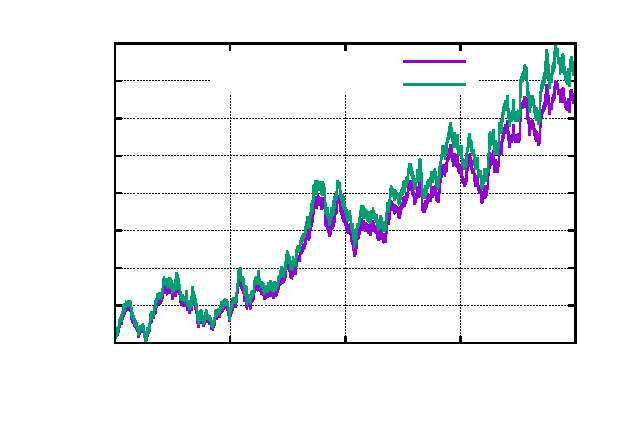
\includegraphics{BadNorm}}%
    \gplfronttext
  \end{picture}%
\endgroup

\end{figure}
}

\frame{
\frametitle{Flipped Normalization}
\begin{figure}
% GNUPLOT: LaTeX picture with Postscript
\begingroup
  \makeatletter
  \providecommand\color[2][]{%
    \GenericError{(gnuplot) \space\space\space\@spaces}{%
      Package color not loaded in conjunction with
      terminal option `colourtext'%
    }{See the gnuplot documentation for explanation.%
    }{Either use 'blacktext' in gnuplot or load the package
      color.sty in LaTeX.}%
    \renewcommand\color[2][]{}%
  }%
  \providecommand\includegraphics[2][]{%
    \GenericError{(gnuplot) \space\space\space\@spaces}{%
      Package graphicx or graphics not loaded%
    }{See the gnuplot documentation for explanation.%
    }{The gnuplot epslatex terminal needs graphicx.sty or graphics.sty.}%
    \renewcommand\includegraphics[2][]{}%
  }%
  \providecommand\rotatebox[2]{#2}%
  \@ifundefined{ifGPcolor}{%
    \newif\ifGPcolor
    \GPcolortrue
  }{}%
  \@ifundefined{ifGPblacktext}{%
    \newif\ifGPblacktext
    \GPblacktexttrue
  }{}%
  % define a \g@addto@macro without @ in the name:
  \let\gplgaddtomacro\g@addto@macro
  % define empty templates for all commands taking text:
  \gdef\gplbacktext{}%
  \gdef\gplfronttext{}%
  \makeatother
  \ifGPblacktext
    % no textcolor at all
    \def\colorrgb#1{}%
    \def\colorgray#1{}%
  \else
    % gray or color?
    \ifGPcolor
      \def\colorrgb#1{\color[rgb]{#1}}%
      \def\colorgray#1{\color[gray]{#1}}%
      \expandafter\def\csname LTw\endcsname{\color{white}}%
      \expandafter\def\csname LTb\endcsname{\color{black}}%
      \expandafter\def\csname LTa\endcsname{\color{black}}%
      \expandafter\def\csname LT0\endcsname{\color[rgb]{1,0,0}}%
      \expandafter\def\csname LT1\endcsname{\color[rgb]{0,1,0}}%
      \expandafter\def\csname LT2\endcsname{\color[rgb]{0,0,1}}%
      \expandafter\def\csname LT3\endcsname{\color[rgb]{1,0,1}}%
      \expandafter\def\csname LT4\endcsname{\color[rgb]{0,1,1}}%
      \expandafter\def\csname LT5\endcsname{\color[rgb]{1,1,0}}%
      \expandafter\def\csname LT6\endcsname{\color[rgb]{0,0,0}}%
      \expandafter\def\csname LT7\endcsname{\color[rgb]{1,0.3,0}}%
      \expandafter\def\csname LT8\endcsname{\color[rgb]{0.5,0.5,0.5}}%
    \else
      % gray
      \def\colorrgb#1{\color{black}}%
      \def\colorgray#1{\color[gray]{#1}}%
      \expandafter\def\csname LTw\endcsname{\color{white}}%
      \expandafter\def\csname LTb\endcsname{\color{black}}%
      \expandafter\def\csname LTa\endcsname{\color{black}}%
      \expandafter\def\csname LT0\endcsname{\color{black}}%
      \expandafter\def\csname LT1\endcsname{\color{black}}%
      \expandafter\def\csname LT2\endcsname{\color{black}}%
      \expandafter\def\csname LT3\endcsname{\color{black}}%
      \expandafter\def\csname LT4\endcsname{\color{black}}%
      \expandafter\def\csname LT5\endcsname{\color{black}}%
      \expandafter\def\csname LT6\endcsname{\color{black}}%
      \expandafter\def\csname LT7\endcsname{\color{black}}%
      \expandafter\def\csname LT8\endcsname{\color{black}}%
    \fi
  \fi
    \setlength{\unitlength}{0.0500bp}%
    \ifx\gptboxheight\undefined%
      \newlength{\gptboxheight}%
      \newlength{\gptboxwidth}%
      \newsavebox{\gptboxtext}%
    \fi%
    \setlength{\fboxrule}{0.5pt}%
    \setlength{\fboxsep}{1pt}%
\begin{picture}(5760.00,3844.00)%
    \gplgaddtomacro\gplbacktext{%
      \csname LTb\endcsname%
      \put(814,704){\makebox(0,0)[r]{\strut{}$0$}}%
      \csname LTb\endcsname%
      \put(814,1063){\makebox(0,0)[r]{\strut{}$0.1$}}%
      \csname LTb\endcsname%
      \put(814,1423){\makebox(0,0)[r]{\strut{}$0.2$}}%
      \csname LTb\endcsname%
      \put(814,1782){\makebox(0,0)[r]{\strut{}$0.3$}}%
      \csname LTb\endcsname%
      \put(814,2142){\makebox(0,0)[r]{\strut{}$0.4$}}%
      \csname LTb\endcsname%
      \put(814,2501){\makebox(0,0)[r]{\strut{}$0.5$}}%
      \csname LTb\endcsname%
      \put(814,2860){\makebox(0,0)[r]{\strut{}$0.6$}}%
      \csname LTb\endcsname%
      \put(814,3220){\makebox(0,0)[r]{\strut{}$0.7$}}%
      \csname LTb\endcsname%
      \put(814,3579){\makebox(0,0)[r]{\strut{}$0.8$}}%
      \csname LTb\endcsname%
      \put(946,484){\makebox(0,0){\strut{}$0$}}%
      \csname LTb\endcsname%
      \put(2050,484){\makebox(0,0){\strut{}$5000$}}%
      \csname LTb\endcsname%
      \put(3155,484){\makebox(0,0){\strut{}$10000$}}%
      \csname LTb\endcsname%
      \put(4259,484){\makebox(0,0){\strut{}$15000$}}%
      \csname LTb\endcsname%
      \put(5363,484){\makebox(0,0){\strut{}$20000$}}%
    }%
    \gplgaddtomacro\gplfronttext{%
      \csname LTb\endcsname%
      \put(176,2141){\rotatebox{-270}{\makebox(0,0){\strut{}Stock Price}}}%
      \put(3154,154){\makebox(0,0){\strut{}Time (Days)}}%
      \csname LTb\endcsname%
      \put(3585,3406){\makebox(0,0)[r]{\strut{}Prediction}}%
      \csname LTb\endcsname%
      \put(3585,3186){\makebox(0,0)[r]{\strut{}Training Data}}%
    }%
    \gplbacktext
    \put(0,0){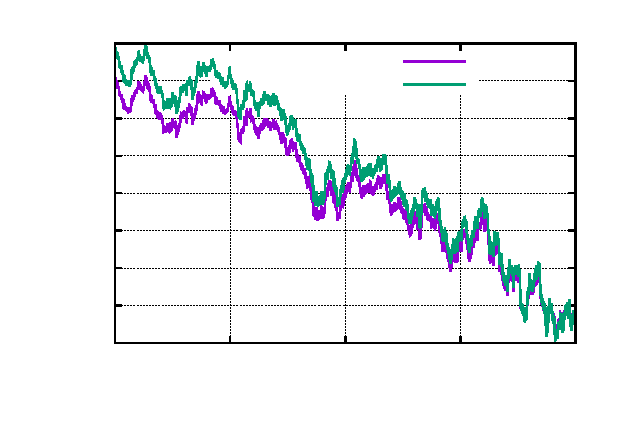
\includegraphics{GoodNorm}}%
    \gplfronttext
  \end{picture}%
\endgroup

\end{figure}
}

\section{Results}

\frame{
\frametitle{Google}
\begin{figure}
% GNUPLOT: LaTeX picture with Postscript
\begingroup
  \makeatletter
  \providecommand\color[2][]{%
    \GenericError{(gnuplot) \space\space\space\@spaces}{%
      Package color not loaded in conjunction with
      terminal option `colourtext'%
    }{See the gnuplot documentation for explanation.%
    }{Either use 'blacktext' in gnuplot or load the package
      color.sty in LaTeX.}%
    \renewcommand\color[2][]{}%
  }%
  \providecommand\includegraphics[2][]{%
    \GenericError{(gnuplot) \space\space\space\@spaces}{%
      Package graphicx or graphics not loaded%
    }{See the gnuplot documentation for explanation.%
    }{The gnuplot epslatex terminal needs graphicx.sty or graphics.sty.}%
    \renewcommand\includegraphics[2][]{}%
  }%
  \providecommand\rotatebox[2]{#2}%
  \@ifundefined{ifGPcolor}{%
    \newif\ifGPcolor
    \GPcolortrue
  }{}%
  \@ifundefined{ifGPblacktext}{%
    \newif\ifGPblacktext
    \GPblacktexttrue
  }{}%
  % define a \g@addto@macro without @ in the name:
  \let\gplgaddtomacro\g@addto@macro
  % define empty templates for all commands taking text:
  \gdef\gplbacktext{}%
  \gdef\gplfronttext{}%
  \makeatother
  \ifGPblacktext
    % no textcolor at all
    \def\colorrgb#1{}%
    \def\colorgray#1{}%
  \else
    % gray or color?
    \ifGPcolor
      \def\colorrgb#1{\color[rgb]{#1}}%
      \def\colorgray#1{\color[gray]{#1}}%
      \expandafter\def\csname LTw\endcsname{\color{white}}%
      \expandafter\def\csname LTb\endcsname{\color{black}}%
      \expandafter\def\csname LTa\endcsname{\color{black}}%
      \expandafter\def\csname LT0\endcsname{\color[rgb]{1,0,0}}%
      \expandafter\def\csname LT1\endcsname{\color[rgb]{0,1,0}}%
      \expandafter\def\csname LT2\endcsname{\color[rgb]{0,0,1}}%
      \expandafter\def\csname LT3\endcsname{\color[rgb]{1,0,1}}%
      \expandafter\def\csname LT4\endcsname{\color[rgb]{0,1,1}}%
      \expandafter\def\csname LT5\endcsname{\color[rgb]{1,1,0}}%
      \expandafter\def\csname LT6\endcsname{\color[rgb]{0,0,0}}%
      \expandafter\def\csname LT7\endcsname{\color[rgb]{1,0.3,0}}%
      \expandafter\def\csname LT8\endcsname{\color[rgb]{0.5,0.5,0.5}}%
    \else
      % gray
      \def\colorrgb#1{\color{black}}%
      \def\colorgray#1{\color[gray]{#1}}%
      \expandafter\def\csname LTw\endcsname{\color{white}}%
      \expandafter\def\csname LTb\endcsname{\color{black}}%
      \expandafter\def\csname LTa\endcsname{\color{black}}%
      \expandafter\def\csname LT0\endcsname{\color{black}}%
      \expandafter\def\csname LT1\endcsname{\color{black}}%
      \expandafter\def\csname LT2\endcsname{\color{black}}%
      \expandafter\def\csname LT3\endcsname{\color{black}}%
      \expandafter\def\csname LT4\endcsname{\color{black}}%
      \expandafter\def\csname LT5\endcsname{\color{black}}%
      \expandafter\def\csname LT6\endcsname{\color{black}}%
      \expandafter\def\csname LT7\endcsname{\color{black}}%
      \expandafter\def\csname LT8\endcsname{\color{black}}%
    \fi
  \fi
    \setlength{\unitlength}{0.0500bp}%
    \ifx\gptboxheight\undefined%
      \newlength{\gptboxheight}%
      \newlength{\gptboxwidth}%
      \newsavebox{\gptboxtext}%
    \fi%
    \setlength{\fboxrule}{0.5pt}%
    \setlength{\fboxsep}{1pt}%
\begin{picture}(5760.00,3844.00)%
    \gplgaddtomacro\gplbacktext{%
      \csname LTb\endcsname%
      \put(946,704){\makebox(0,0)[r]{\strut{}$900$}}%
      \csname LTb\endcsname%
      \put(946,1063){\makebox(0,0)[r]{\strut{}$920$}}%
      \csname LTb\endcsname%
      \put(946,1423){\makebox(0,0)[r]{\strut{}$940$}}%
      \csname LTb\endcsname%
      \put(946,1782){\makebox(0,0)[r]{\strut{}$960$}}%
      \csname LTb\endcsname%
      \put(946,2142){\makebox(0,0)[r]{\strut{}$980$}}%
      \csname LTb\endcsname%
      \put(946,2501){\makebox(0,0)[r]{\strut{}$1000$}}%
      \csname LTb\endcsname%
      \put(946,2860){\makebox(0,0)[r]{\strut{}$1020$}}%
      \csname LTb\endcsname%
      \put(946,3220){\makebox(0,0)[r]{\strut{}$1040$}}%
      \csname LTb\endcsname%
      \put(946,3579){\makebox(0,0)[r]{\strut{}$1060$}}%
      \csname LTb\endcsname%
      \put(1078,484){\makebox(0,0){\strut{}$-90$}}%
      \csname LTb\endcsname%
      \put(1554,484){\makebox(0,0){\strut{}$-80$}}%
      \csname LTb\endcsname%
      \put(2030,484){\makebox(0,0){\strut{}$-70$}}%
      \csname LTb\endcsname%
      \put(2506,484){\makebox(0,0){\strut{}$-60$}}%
      \csname LTb\endcsname%
      \put(2982,484){\makebox(0,0){\strut{}$-50$}}%
      \csname LTb\endcsname%
      \put(3459,484){\makebox(0,0){\strut{}$-40$}}%
      \csname LTb\endcsname%
      \put(3935,484){\makebox(0,0){\strut{}$-30$}}%
      \csname LTb\endcsname%
      \put(4411,484){\makebox(0,0){\strut{}$-20$}}%
      \csname LTb\endcsname%
      \put(4887,484){\makebox(0,0){\strut{}$-10$}}%
      \csname LTb\endcsname%
      \put(5363,484){\makebox(0,0){\strut{}$0$}}%
    }%
    \gplgaddtomacro\gplfronttext{%
      \csname LTb\endcsname%
      \put(176,2141){\rotatebox{-270}{\makebox(0,0){\strut{}Stock Price}}}%
      \put(3220,154){\makebox(0,0){\strut{}Time (Days)}}%
      \csname LTb\endcsname%
      \put(2530,3406){\makebox(0,0)[r]{\strut{}Prediction}}%
      \csname LTb\endcsname%
      \put(2530,3186){\makebox(0,0)[r]{\strut{}Google}}%
    }%
    \gplbacktext
    \put(0,0){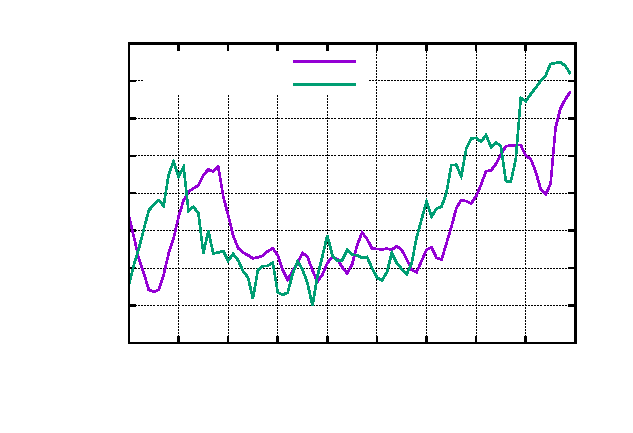
\includegraphics{Google}}%
    \gplfronttext
  \end{picture}%
\endgroup

\end{figure}
}

\frame{
\frametitle{Apple}
\begin{figure}
% GNUPLOT: LaTeX picture with Postscript
\begingroup
  \makeatletter
  \providecommand\color[2][]{%
    \GenericError{(gnuplot) \space\space\space\@spaces}{%
      Package color not loaded in conjunction with
      terminal option `colourtext'%
    }{See the gnuplot documentation for explanation.%
    }{Either use 'blacktext' in gnuplot or load the package
      color.sty in LaTeX.}%
    \renewcommand\color[2][]{}%
  }%
  \providecommand\includegraphics[2][]{%
    \GenericError{(gnuplot) \space\space\space\@spaces}{%
      Package graphicx or graphics not loaded%
    }{See the gnuplot documentation for explanation.%
    }{The gnuplot epslatex terminal needs graphicx.sty or graphics.sty.}%
    \renewcommand\includegraphics[2][]{}%
  }%
  \providecommand\rotatebox[2]{#2}%
  \@ifundefined{ifGPcolor}{%
    \newif\ifGPcolor
    \GPcolortrue
  }{}%
  \@ifundefined{ifGPblacktext}{%
    \newif\ifGPblacktext
    \GPblacktexttrue
  }{}%
  % define a \g@addto@macro without @ in the name:
  \let\gplgaddtomacro\g@addto@macro
  % define empty templates for all commands taking text:
  \gdef\gplbacktext{}%
  \gdef\gplfronttext{}%
  \makeatother
  \ifGPblacktext
    % no textcolor at all
    \def\colorrgb#1{}%
    \def\colorgray#1{}%
  \else
    % gray or color?
    \ifGPcolor
      \def\colorrgb#1{\color[rgb]{#1}}%
      \def\colorgray#1{\color[gray]{#1}}%
      \expandafter\def\csname LTw\endcsname{\color{white}}%
      \expandafter\def\csname LTb\endcsname{\color{black}}%
      \expandafter\def\csname LTa\endcsname{\color{black}}%
      \expandafter\def\csname LT0\endcsname{\color[rgb]{1,0,0}}%
      \expandafter\def\csname LT1\endcsname{\color[rgb]{0,1,0}}%
      \expandafter\def\csname LT2\endcsname{\color[rgb]{0,0,1}}%
      \expandafter\def\csname LT3\endcsname{\color[rgb]{1,0,1}}%
      \expandafter\def\csname LT4\endcsname{\color[rgb]{0,1,1}}%
      \expandafter\def\csname LT5\endcsname{\color[rgb]{1,1,0}}%
      \expandafter\def\csname LT6\endcsname{\color[rgb]{0,0,0}}%
      \expandafter\def\csname LT7\endcsname{\color[rgb]{1,0.3,0}}%
      \expandafter\def\csname LT8\endcsname{\color[rgb]{0.5,0.5,0.5}}%
    \else
      % gray
      \def\colorrgb#1{\color{black}}%
      \def\colorgray#1{\color[gray]{#1}}%
      \expandafter\def\csname LTw\endcsname{\color{white}}%
      \expandafter\def\csname LTb\endcsname{\color{black}}%
      \expandafter\def\csname LTa\endcsname{\color{black}}%
      \expandafter\def\csname LT0\endcsname{\color{black}}%
      \expandafter\def\csname LT1\endcsname{\color{black}}%
      \expandafter\def\csname LT2\endcsname{\color{black}}%
      \expandafter\def\csname LT3\endcsname{\color{black}}%
      \expandafter\def\csname LT4\endcsname{\color{black}}%
      \expandafter\def\csname LT5\endcsname{\color{black}}%
      \expandafter\def\csname LT6\endcsname{\color{black}}%
      \expandafter\def\csname LT7\endcsname{\color{black}}%
      \expandafter\def\csname LT8\endcsname{\color{black}}%
    \fi
  \fi
    \setlength{\unitlength}{0.0500bp}%
    \ifx\gptboxheight\undefined%
      \newlength{\gptboxheight}%
      \newlength{\gptboxwidth}%
      \newsavebox{\gptboxtext}%
    \fi%
    \setlength{\fboxrule}{0.5pt}%
    \setlength{\fboxsep}{1pt}%
\begin{picture}(5760.00,3844.00)%
    \gplgaddtomacro\gplbacktext{%
      \csname LTb\endcsname%
      \put(814,704){\makebox(0,0)[r]{\strut{}$145$}}%
      \csname LTb\endcsname%
      \put(814,1115){\makebox(0,0)[r]{\strut{}$150$}}%
      \csname LTb\endcsname%
      \put(814,1525){\makebox(0,0)[r]{\strut{}$155$}}%
      \csname LTb\endcsname%
      \put(814,1936){\makebox(0,0)[r]{\strut{}$160$}}%
      \csname LTb\endcsname%
      \put(814,2347){\makebox(0,0)[r]{\strut{}$165$}}%
      \csname LTb\endcsname%
      \put(814,2758){\makebox(0,0)[r]{\strut{}$170$}}%
      \csname LTb\endcsname%
      \put(814,3168){\makebox(0,0)[r]{\strut{}$175$}}%
      \csname LTb\endcsname%
      \put(814,3579){\makebox(0,0)[r]{\strut{}$180$}}%
      \csname LTb\endcsname%
      \put(946,484){\makebox(0,0){\strut{}$-90$}}%
      \csname LTb\endcsname%
      \put(1437,484){\makebox(0,0){\strut{}$-80$}}%
      \csname LTb\endcsname%
      \put(1928,484){\makebox(0,0){\strut{}$-70$}}%
      \csname LTb\endcsname%
      \put(2418,484){\makebox(0,0){\strut{}$-60$}}%
      \csname LTb\endcsname%
      \put(2909,484){\makebox(0,0){\strut{}$-50$}}%
      \csname LTb\endcsname%
      \put(3400,484){\makebox(0,0){\strut{}$-40$}}%
      \csname LTb\endcsname%
      \put(3891,484){\makebox(0,0){\strut{}$-30$}}%
      \csname LTb\endcsname%
      \put(4381,484){\makebox(0,0){\strut{}$-20$}}%
      \csname LTb\endcsname%
      \put(4872,484){\makebox(0,0){\strut{}$-10$}}%
      \csname LTb\endcsname%
      \put(5363,484){\makebox(0,0){\strut{}$0$}}%
    }%
    \gplgaddtomacro\gplfronttext{%
      \csname LTb\endcsname%
      \put(176,2141){\rotatebox{-270}{\makebox(0,0){\strut{}Stock Price}}}%
      \put(3154,154){\makebox(0,0){\strut{}Time (Days)}}%
      \csname LTb\endcsname%
      \put(2398,3406){\makebox(0,0)[r]{\strut{}Prediction}}%
      \csname LTb\endcsname%
      \put(2398,3186){\makebox(0,0)[r]{\strut{}Apple}}%
    }%
    \gplbacktext
    \put(0,0){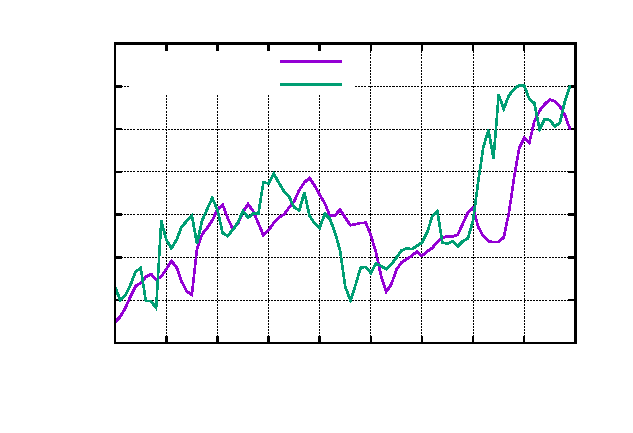
\includegraphics{Apple}}%
    \gplfronttext
  \end{picture}%
\endgroup

\end{figure}
}

\frame{
\frametitle{Absolute Difference}
\begin{figure}
% GNUPLOT: LaTeX picture with Postscript
\begingroup
  \makeatletter
  \providecommand\color[2][]{%
    \GenericError{(gnuplot) \space\space\space\@spaces}{%
      Package color not loaded in conjunction with
      terminal option `colourtext'%
    }{See the gnuplot documentation for explanation.%
    }{Either use 'blacktext' in gnuplot or load the package
      color.sty in LaTeX.}%
    \renewcommand\color[2][]{}%
  }%
  \providecommand\includegraphics[2][]{%
    \GenericError{(gnuplot) \space\space\space\@spaces}{%
      Package graphicx or graphics not loaded%
    }{See the gnuplot documentation for explanation.%
    }{The gnuplot epslatex terminal needs graphicx.sty or graphics.sty.}%
    \renewcommand\includegraphics[2][]{}%
  }%
  \providecommand\rotatebox[2]{#2}%
  \@ifundefined{ifGPcolor}{%
    \newif\ifGPcolor
    \GPcolortrue
  }{}%
  \@ifundefined{ifGPblacktext}{%
    \newif\ifGPblacktext
    \GPblacktexttrue
  }{}%
  % define a \g@addto@macro without @ in the name:
  \let\gplgaddtomacro\g@addto@macro
  % define empty templates for all commands taking text:
  \gdef\gplbacktext{}%
  \gdef\gplfronttext{}%
  \makeatother
  \ifGPblacktext
    % no textcolor at all
    \def\colorrgb#1{}%
    \def\colorgray#1{}%
  \else
    % gray or color?
    \ifGPcolor
      \def\colorrgb#1{\color[rgb]{#1}}%
      \def\colorgray#1{\color[gray]{#1}}%
      \expandafter\def\csname LTw\endcsname{\color{white}}%
      \expandafter\def\csname LTb\endcsname{\color{black}}%
      \expandafter\def\csname LTa\endcsname{\color{black}}%
      \expandafter\def\csname LT0\endcsname{\color[rgb]{1,0,0}}%
      \expandafter\def\csname LT1\endcsname{\color[rgb]{0,1,0}}%
      \expandafter\def\csname LT2\endcsname{\color[rgb]{0,0,1}}%
      \expandafter\def\csname LT3\endcsname{\color[rgb]{1,0,1}}%
      \expandafter\def\csname LT4\endcsname{\color[rgb]{0,1,1}}%
      \expandafter\def\csname LT5\endcsname{\color[rgb]{1,1,0}}%
      \expandafter\def\csname LT6\endcsname{\color[rgb]{0,0,0}}%
      \expandafter\def\csname LT7\endcsname{\color[rgb]{1,0.3,0}}%
      \expandafter\def\csname LT8\endcsname{\color[rgb]{0.5,0.5,0.5}}%
    \else
      % gray
      \def\colorrgb#1{\color{black}}%
      \def\colorgray#1{\color[gray]{#1}}%
      \expandafter\def\csname LTw\endcsname{\color{white}}%
      \expandafter\def\csname LTb\endcsname{\color{black}}%
      \expandafter\def\csname LTa\endcsname{\color{black}}%
      \expandafter\def\csname LT0\endcsname{\color{black}}%
      \expandafter\def\csname LT1\endcsname{\color{black}}%
      \expandafter\def\csname LT2\endcsname{\color{black}}%
      \expandafter\def\csname LT3\endcsname{\color{black}}%
      \expandafter\def\csname LT4\endcsname{\color{black}}%
      \expandafter\def\csname LT5\endcsname{\color{black}}%
      \expandafter\def\csname LT6\endcsname{\color{black}}%
      \expandafter\def\csname LT7\endcsname{\color{black}}%
      \expandafter\def\csname LT8\endcsname{\color{black}}%
    \fi
  \fi
    \setlength{\unitlength}{0.0500bp}%
    \ifx\gptboxheight\undefined%
      \newlength{\gptboxheight}%
      \newlength{\gptboxwidth}%
      \newsavebox{\gptboxtext}%
    \fi%
    \setlength{\fboxrule}{0.5pt}%
    \setlength{\fboxsep}{1pt}%
\begin{picture}(5760.00,3844.00)%
    \gplgaddtomacro\gplbacktext{%
      \csname LTb\endcsname%
      \put(814,704){\makebox(0,0)[r]{\strut{}$-80$}}%
      \csname LTb\endcsname%
      \put(814,1115){\makebox(0,0)[r]{\strut{}$-60$}}%
      \csname LTb\endcsname%
      \put(814,1525){\makebox(0,0)[r]{\strut{}$-40$}}%
      \csname LTb\endcsname%
      \put(814,1936){\makebox(0,0)[r]{\strut{}$-20$}}%
      \csname LTb\endcsname%
      \put(814,2347){\makebox(0,0)[r]{\strut{}$0$}}%
      \csname LTb\endcsname%
      \put(814,2758){\makebox(0,0)[r]{\strut{}$20$}}%
      \csname LTb\endcsname%
      \put(814,3168){\makebox(0,0)[r]{\strut{}$40$}}%
      \csname LTb\endcsname%
      \put(814,3579){\makebox(0,0)[r]{\strut{}$60$}}%
      \csname LTb\endcsname%
      \put(946,484){\makebox(0,0){\strut{}$-90$}}%
      \csname LTb\endcsname%
      \put(1437,484){\makebox(0,0){\strut{}$-80$}}%
      \csname LTb\endcsname%
      \put(1928,484){\makebox(0,0){\strut{}$-70$}}%
      \csname LTb\endcsname%
      \put(2418,484){\makebox(0,0){\strut{}$-60$}}%
      \csname LTb\endcsname%
      \put(2909,484){\makebox(0,0){\strut{}$-50$}}%
      \csname LTb\endcsname%
      \put(3400,484){\makebox(0,0){\strut{}$-40$}}%
      \csname LTb\endcsname%
      \put(3891,484){\makebox(0,0){\strut{}$-30$}}%
      \csname LTb\endcsname%
      \put(4381,484){\makebox(0,0){\strut{}$-20$}}%
      \csname LTb\endcsname%
      \put(4872,484){\makebox(0,0){\strut{}$-10$}}%
      \csname LTb\endcsname%
      \put(5363,484){\makebox(0,0){\strut{}$0$}}%
    }%
    \gplgaddtomacro\gplfronttext{%
      \csname LTb\endcsname%
      \put(176,2141){\rotatebox{-270}{\makebox(0,0){\strut{}Absolute Difference}}}%
      \put(3154,154){\makebox(0,0){\strut{}Time (Days)}}%
      \csname LTb\endcsname%
      \put(1870,1097){\makebox(0,0)[r]{\strut{}Google}}%
      \csname LTb\endcsname%
      \put(1870,877){\makebox(0,0)[r]{\strut{}Apple}}%
    }%
    \gplbacktext
    \put(0,0){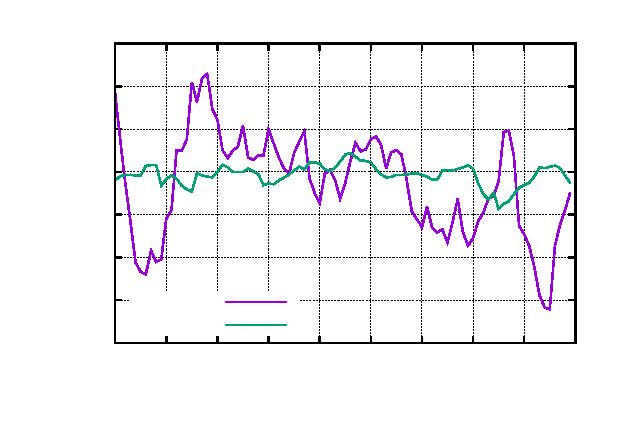
\includegraphics{diff}}%
    \gplfronttext
  \end{picture}%
\endgroup

\end{figure}
}

\frame{
\frametitle{Percent Difference}
\begin{figure}
% GNUPLOT: LaTeX picture with Postscript
\begingroup
  \makeatletter
  \providecommand\color[2][]{%
    \GenericError{(gnuplot) \space\space\space\@spaces}{%
      Package color not loaded in conjunction with
      terminal option `colourtext'%
    }{See the gnuplot documentation for explanation.%
    }{Either use 'blacktext' in gnuplot or load the package
      color.sty in LaTeX.}%
    \renewcommand\color[2][]{}%
  }%
  \providecommand\includegraphics[2][]{%
    \GenericError{(gnuplot) \space\space\space\@spaces}{%
      Package graphicx or graphics not loaded%
    }{See the gnuplot documentation for explanation.%
    }{The gnuplot epslatex terminal needs graphicx.sty or graphics.sty.}%
    \renewcommand\includegraphics[2][]{}%
  }%
  \providecommand\rotatebox[2]{#2}%
  \@ifundefined{ifGPcolor}{%
    \newif\ifGPcolor
    \GPcolortrue
  }{}%
  \@ifundefined{ifGPblacktext}{%
    \newif\ifGPblacktext
    \GPblacktexttrue
  }{}%
  % define a \g@addto@macro without @ in the name:
  \let\gplgaddtomacro\g@addto@macro
  % define empty templates for all commands taking text:
  \gdef\gplbacktext{}%
  \gdef\gplfronttext{}%
  \makeatother
  \ifGPblacktext
    % no textcolor at all
    \def\colorrgb#1{}%
    \def\colorgray#1{}%
  \else
    % gray or color?
    \ifGPcolor
      \def\colorrgb#1{\color[rgb]{#1}}%
      \def\colorgray#1{\color[gray]{#1}}%
      \expandafter\def\csname LTw\endcsname{\color{white}}%
      \expandafter\def\csname LTb\endcsname{\color{black}}%
      \expandafter\def\csname LTa\endcsname{\color{black}}%
      \expandafter\def\csname LT0\endcsname{\color[rgb]{1,0,0}}%
      \expandafter\def\csname LT1\endcsname{\color[rgb]{0,1,0}}%
      \expandafter\def\csname LT2\endcsname{\color[rgb]{0,0,1}}%
      \expandafter\def\csname LT3\endcsname{\color[rgb]{1,0,1}}%
      \expandafter\def\csname LT4\endcsname{\color[rgb]{0,1,1}}%
      \expandafter\def\csname LT5\endcsname{\color[rgb]{1,1,0}}%
      \expandafter\def\csname LT6\endcsname{\color[rgb]{0,0,0}}%
      \expandafter\def\csname LT7\endcsname{\color[rgb]{1,0.3,0}}%
      \expandafter\def\csname LT8\endcsname{\color[rgb]{0.5,0.5,0.5}}%
    \else
      % gray
      \def\colorrgb#1{\color{black}}%
      \def\colorgray#1{\color[gray]{#1}}%
      \expandafter\def\csname LTw\endcsname{\color{white}}%
      \expandafter\def\csname LTb\endcsname{\color{black}}%
      \expandafter\def\csname LTa\endcsname{\color{black}}%
      \expandafter\def\csname LT0\endcsname{\color{black}}%
      \expandafter\def\csname LT1\endcsname{\color{black}}%
      \expandafter\def\csname LT2\endcsname{\color{black}}%
      \expandafter\def\csname LT3\endcsname{\color{black}}%
      \expandafter\def\csname LT4\endcsname{\color{black}}%
      \expandafter\def\csname LT5\endcsname{\color{black}}%
      \expandafter\def\csname LT6\endcsname{\color{black}}%
      \expandafter\def\csname LT7\endcsname{\color{black}}%
      \expandafter\def\csname LT8\endcsname{\color{black}}%
    \fi
  \fi
    \setlength{\unitlength}{0.0500bp}%
    \ifx\gptboxheight\undefined%
      \newlength{\gptboxheight}%
      \newlength{\gptboxwidth}%
      \newsavebox{\gptboxtext}%
    \fi%
    \setlength{\fboxrule}{0.5pt}%
    \setlength{\fboxsep}{1pt}%
\begin{picture}(5760.00,3844.00)%
    \gplgaddtomacro\gplbacktext{%
      \csname LTb\endcsname%
      \put(1078,704){\makebox(0,0)[r]{\strut{}$-0.1$}}%
      \csname LTb\endcsname%
      \put(1078,1063){\makebox(0,0)[r]{\strut{}$-0.08$}}%
      \csname LTb\endcsname%
      \put(1078,1423){\makebox(0,0)[r]{\strut{}$-0.06$}}%
      \csname LTb\endcsname%
      \put(1078,1782){\makebox(0,0)[r]{\strut{}$-0.04$}}%
      \csname LTb\endcsname%
      \put(1078,2142){\makebox(0,0)[r]{\strut{}$-0.02$}}%
      \csname LTb\endcsname%
      \put(1078,2501){\makebox(0,0)[r]{\strut{}$0$}}%
      \csname LTb\endcsname%
      \put(1078,2860){\makebox(0,0)[r]{\strut{}$0.02$}}%
      \csname LTb\endcsname%
      \put(1078,3220){\makebox(0,0)[r]{\strut{}$0.04$}}%
      \csname LTb\endcsname%
      \put(1078,3579){\makebox(0,0)[r]{\strut{}$0.06$}}%
      \csname LTb\endcsname%
      \put(1210,484){\makebox(0,0){\strut{}$-90$}}%
      \csname LTb\endcsname%
      \put(1671,484){\makebox(0,0){\strut{}$-80$}}%
      \csname LTb\endcsname%
      \put(2133,484){\makebox(0,0){\strut{}$-70$}}%
      \csname LTb\endcsname%
      \put(2594,484){\makebox(0,0){\strut{}$-60$}}%
      \csname LTb\endcsname%
      \put(3056,484){\makebox(0,0){\strut{}$-50$}}%
      \csname LTb\endcsname%
      \put(3517,484){\makebox(0,0){\strut{}$-40$}}%
      \csname LTb\endcsname%
      \put(3979,484){\makebox(0,0){\strut{}$-30$}}%
      \csname LTb\endcsname%
      \put(4440,484){\makebox(0,0){\strut{}$-20$}}%
      \csname LTb\endcsname%
      \put(4902,484){\makebox(0,0){\strut{}$-10$}}%
      \csname LTb\endcsname%
      \put(5363,484){\makebox(0,0){\strut{}$0$}}%
    }%
    \gplgaddtomacro\gplfronttext{%
      \csname LTb\endcsname%
      \put(176,2141){\rotatebox{-270}{\makebox(0,0){\strut{}Percent Difference}}}%
      \put(3286,154){\makebox(0,0){\strut{}Time (Days)}}%
      \csname LTb\endcsname%
      \put(2134,1097){\makebox(0,0)[r]{\strut{}Google}}%
      \csname LTb\endcsname%
      \put(2134,877){\makebox(0,0)[r]{\strut{}Apple}}%
    }%
    \gplbacktext
    \put(0,0){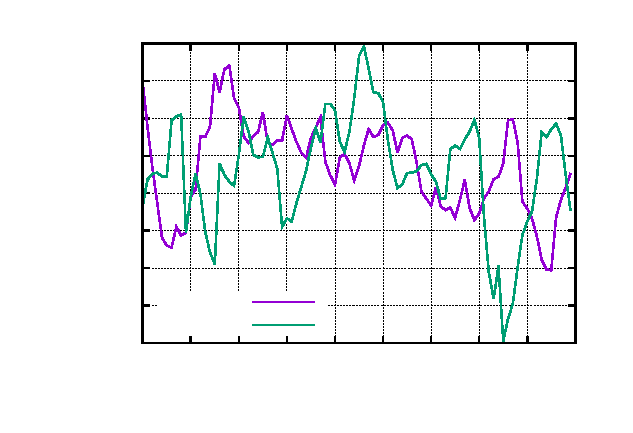
\includegraphics{Percent}}%
    \gplfronttext
  \end{picture}%
\endgroup

\end{figure}
}

\frame{
\frametitle{Conclusion}
This model can predict stock prices within about 2\%, however, this is more than the day-to-day fluctuations. Moreover, the prediction seems to lag behind the stock by approximately a week, and so it is probably unwise to invest money based this model.
}

\end{document}
